% This work is licensed under the Creative Commons Attribution-NonCommercial-NoDerivs
% 3.0 Unported License. To view a copy of this license, visit
% http://creativecommons.org/licenses/by-nc-nd/3.0/ or send a letter to
% Creative Commons, 444 Castro Street, Suite 900, Mountain View, California, 94041, USA.

\documentclass{beamer}

\usepackage[utf8x]{inputenc}
% \usetheme{Excilys}
\usetheme{CambridgeUS}

% rappel du plan à chaque partie
\AtBeginSection[]
{
  \begin{frame}<beamer>\frametitle{Plan}
    \frametitle{}
    \tableofcontents[hideothersubsections,currentsection]
  \end{frame}
}

% n° de ligne en bas
% \defbeamertemplate*{footline}{infolines theme}
% {
% \begin{beamercolorbox}{date in head/foot}%
% \centering
% {
  % \insertframenumber{} / \inserttotalframenumber
% }
% \end{beamercolorbox}%
% }%

% se débarasse des symboles de navigation en bas de la page
\setbeamertemplate{navigation symbols}{}


\title{Formation git}
\author{Groupe Excilys}

\begin{document}
%-------------------------------------------------------------------------------
% This work is licensed under the Creative Commons Attribution-NonCommercial-NoDerivs
% 3.0 Unported License. To view a copy of this license, visit
% http://creativecommons.org/licenses/by-nc-nd/3.0/ or send a letter to
% Creative Commons, 444 Castro Street, Suite 900, Mountain View, California, 94041, USA.

\begin{frame}
  \titlepage
\end{frame}

% max 80 columns : merges become messy with pure text and longer lines.
% vim: set colorcolumn=+1 textwidth=80:

%-------------------------------------------------------------------------------
\section*{Introduction}
% This work is licensed under the Creative Commons Attribution-NonCommercial-NoDerivs
% 3.0 Unported License. To view a copy of this license, visit
% http://creativecommons.org/licenses/by-nc-nd/3.0/ or send a letter to
% Creative Commons, 444 Castro Street, Suite 900, Mountain View, California, 94041, USA.

%-------------------------------------------------------------------------------
% TODO : add a "It's dangerous to go alone, take this" picture.
\begin{frame}\frametitle{Caractéristiques}
  \begin{itemize}
    \item initié par Linus Torvalds pour le noyau Linux
    \item architecture distribuée

      \begin{itemize}
        \item pas de dépôt central obligatoire
        \item chaque dépôt peut fonctionner en autarcie
      \end{itemize}

    \item nombre important de commandes
    \item développement non-linéaire facilité

      \begin{itemize}
        \item création/manipulation des branches
      \end{itemize}

    \item efficace quelle que soit la taille du projet

      \begin{itemize}
        \item projets GitHub: Rails, jQuery, Node.js
      \end{itemize}

    \item GNU GPL v2

  \end{itemize}
\end{frame}
%-------------------------------------------------------------------------------

% max 80 columns : merges become messy with pure text and longer lines.
% vim: set colorcolumn=+1 textwidth=80:

%-------------------------------------------------------------------------------
\begin{frame}\frametitle{Plan}
\tableofcontents
\end{frame}
%-------------------------------------------------------------------------------
\section{Travailler en local}
% This work is licensed under the Creative Commons Attribution-NonCommercial-NoDerivs
% 3.0 Unported License. To view a copy of this license, visit
% http://creativecommons.org/licenses/by-nc-nd/3.0/ or send a letter to
% Creative Commons, 444 Castro Street, Suite 900, Mountain View, California, 94041, USA.

%-------------------------------------------------------------------------------
\begin{frame}\frametitle{Résumé des principales commandes}
  cheatsheet: \url{https://github.com/AlexZeitler/gitcheatsheet}
\end{frame}
%-------------------------------------------------------------------------------
\begin{frame}[fragile]\frametitle{Création}

% TODO : faire en // la manip sur un terminal
  \begin{block}{À partir de fichiers locaux}
    \begin{semiverbatim}
\$ \alert{git init}
    \end{semiverbatim}
  \end{block}
  \begin{block}{À partir d'un dépôt existant}
    \begin{semiverbatim}
\$ \alert{git clone git@github.com:excilys/formation-git.git}
    \end{semiverbatim}
  \end{block}

\end{frame}
%-------------------------------------------------------------------------------
\begin{frame}[fragile]\frametitle{Anatomie d'un projet git}
  \begin{semiverbatim}
  \$ \alert{ls -A1}
  formation.tex
  \alert{.git/}
  .gitignore
  images/
  Makefile
  \end{semiverbatim}

  Le .git représente le dépôt git, il contient l'ensemble des
  commits, branches et tags créés.
\end{frame}
%-------------------------------------------------------------------------------
\begin{frame}[fragile]\frametitle{Le fichier .gitignore}
  chemins (fichiers et/ou dossiers) ignorés par git
  \begin{semiverbatim}
  \$ \alert{cat .gitignore}
  .project
  target
  *.iml
  *.ipr
  *.iws
  *.idea
  \end{semiverbatim}

\end{frame}
%-------------------------------------------------------------------------------
\begin{frame}[fragile]\frametitle{Visualisation}
  Historique des commits: \verb|git log|

  \begin{semiverbatim}
  \$ \alert{git log}
  \end{semiverbatim}


  Auteurs des dernières modifications: \alert{git blame}
\end{frame}
%-------------------------------------------------------------------------------
\begin{frame}\frametitle{Staging area (ou Stage)}
  Zone intermédiaire entre l'espace de travail et le dépôt
  \begin{center}
    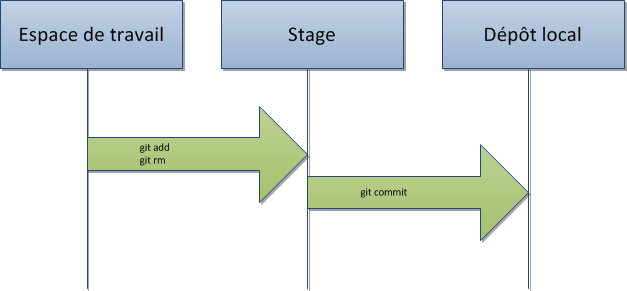
\includegraphics[width=\textwidth]{./images/staging-area.png}
  \end{center}

\end{frame}
%-------------------------------------------------------------------------------
\begin{frame}[fragile]\frametitle{Manipuler la staging area}
  \begin{itemize}
    \item \alert{git add} : ajoute ("stage") un fichier à la staging area
    \item \alert{git rm} : supprime un fichier managé et enregistre sa suppression
      dans la staging area
    \item \alert{git reset HEAD} : retire des modifications de la staging area
  \end{itemize}

  \textit{bonus : git add -p, git add -A}

\end{frame}
%-------------------------------------------------------------------------------
\begin{frame}[fragile]\frametitle{Visualisation}

\begin{semiverbatim}

  \$ \alert{git status}
  # On branch master
  #
  # Changes to be committed:
  #
  modified: some_text.txt \alert{ <-- modifié puis staged}
  #
  # Changes not staged for commit:
  #
  modified: some_more_text.txt \alert{ <-- modifié, non staged}
  #
  \end{semiverbatim}
\end{frame}
  
%-------------------------------------------------------------------------------
\begin{frame}[fragile]\frametitle{Visualisation}
  
\begin{semiverbatim}

  \$ \alert{git diff}  <-- \textbf{modifications non-staged (détail)}
  diff --git a/some_more_text.txt b/some_more_text.txt
  --- a/some_more_text.txt
  +++ b/some_more_text.txt
  +here neither
	
  \$ \alert{git diff --staged}  <-- \textbf{modifications staged (détail)}
  diff --git a/some_text.txt b/some_text.txt
  --- a/some_text.txt
  +++ b/some_text.txt
  +nothing interesting here
\end{semiverbatim}

\end{frame}
%-------------------------------------------------------------------------------
\begin{frame}[fragile]\frametitle{Message de commit}
\begin{block}{Un message bien formé contient :}
  \begin{itemize}
    \item Un titre de moins de 50 caractères
    \item Un paragraphe d'explications (le cas échéant), séparé du titre par une ligne vide, d'une largeur de 72 caractères.
  \end{itemize}
\end{block}

Pour plus d'informations, voir
\url{http://tbaggery.com/2008/04/19/a-note-about-git-commit-messages.html}
\end{frame}
%-------------------------------------------------------------------------------
\begin{frame}\frametitle{Commit}
  Enregistre dans le dépôt local le contenu de la staging area.
  \begin{center}
    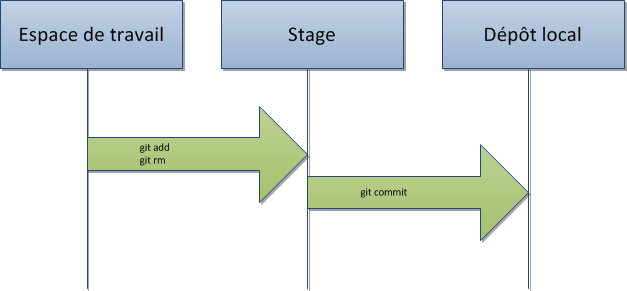
\includegraphics[width=\textwidth]{./images/staging-area.png}
  \end{center}
  Dans git, \alert{commit} a le sens de \textit{coucher par écrit} ou
\textit{acter}.
\end{frame}
%-------------------------------------------------------------------------------

\begin{frame}[fragile]\frametitle{TP : git clone, git log}
  Cloner un projet simple et regarder les commits / logs.
  \note{pas de push, on verra ça dans la partie 2 : avec un seul remote, les
conflits sont inévitables}
\end{frame}
\begin{frame}[fragile]\frametitle{TP : lifecycle simple}
  git init
  add, reset HEAD, commit, rm, etc
  % TODO : schema sur les differents etats des modifs, avec les commandes
\end{frame}
% max 80 columns : merges become messy with pure text and longer lines.
% vim: set colorcolumn=+1 textwidth=80:

%-------------------------------------------------------------------------------
\section{Repository distant}
% This work is licensed under the Creative Commons Attribution-NonCommercial-NoDerivs
% 3.0 Unported License. To view a copy of this license, visit
% http://creativecommons.org/licenses/by-nc-nd/3.0/ or send a letter to
% Creative Commons, 444 Castro Street, Suite 900, Mountain View, California, 94041, USA.

%-------------------------------------------------------------------------------
\begin{frame}[fragile]\frametitle{Mises à jour du dépôt local}
  \begin{itemize}
    \item S'informer des changements distants: \alert{git fetch}
    \item Fetch et appliquer dans le repository local : \alert{git pull}
  \end{itemize}

\end{frame}
%-------------------------------------------------------------------------------
\begin{frame}[fragile]\frametitle{Mises à jour du dépôt local, fast forward}
  \begin{center}
    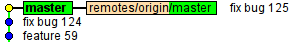
\includegraphics[width=0.8\textwidth]{./images/merge-0.png}
  \end{center}
  \pause
  \hfill
  \begin{center}
    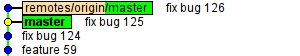
\includegraphics[width=0.8\textwidth]{./images/merge-1.png}
  \end{center}
  \pause
  \hfill
  \begin{center}
    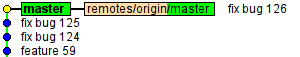
\includegraphics[width=0.8\textwidth]{./images/merge-2.png}
  \end{center}
\end{frame}
%-------------------------------------------------------------------------------
\begin{frame}[fragile]\frametitle{Mises à jour du dépôt local, non fast forward}
  \begin{center}
    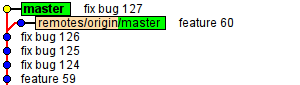
\includegraphics[width=0.8\textwidth]{./images/merge-3.png}
  \end{center}
  \pause
  \hfill
  \begin{center}
    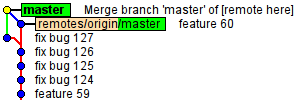
\includegraphics[width=0.8\textwidth]{./images/merge-4.png}
  \end{center}
\end{frame}
%-------------------------------------------------------------------------------
\begin{frame}[fragile]\frametitle{Mises à jour du dépôt distant}
  \alert{git push}
  \hfill
  \begin{center}
    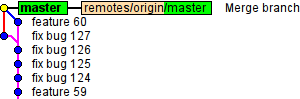
\includegraphics[width=0.8\textwidth]{./images/merge-5.png}
  \end{center}
  \note{attention au push.default, qui a changé avec git 1.7.11}
\end{frame}
%-------------------------------------------------------------------------------
\begin{frame}\frametitle{TP}
  git pull, commit, push
\end{frame}
%-------------------------------------------------------------------------------
% max 80 columns : merges become messy with pure text and longer lines.
% vim: set colorcolumn=+1 textwidth=80:

%-------------------------------------------------------------------------------
\section{Branches}
\begin{frame}[fragile]\frametitle{Les branches dans git}
  Une branche est ...
  \begin{itemize}
  \item Gratuite !
  \note{beaucoup plus simple que sur svn (pas de recopie du projet par exemple)}
  \item Un pointeur vers un commit
  \note{pas un dossier, juste une "etiquette" pointant sur un commit}
  \item merge entre branches facile
  \item utile quelle que soit la durée de vie de cette branche
  \end{itemize}

\end{frame}
%-------------------------------------------------------------------------------
\begin{frame}[fragile]\frametitle{Manipulation de branches}
  \begin{itemize}
  \item Lister toutes les branches: \alert{git branch [-r] [-a]}
  \item Se placer sur une branche: \alert{git checkout [nom\_branche]}
  \item Créer une branche: \alert{git branch [nom\_branche]}
  \item Suivre une branche distante : \alert{git checkout -b [nom\_branche]
  [branche\_distante]}
  \item Supprimer une branche: \alert{git branch -d [nom\_branche]}
  \end{itemize}

\end{frame}
%-------------------------------------------------------------------------------
\begin{frame}[fragile]\frametitle{Cas d'utilisation courants}
  \begin{itemize}
\item développement d'une fonctionnalité
\item correction de bug
\item branche de maintenance
  \end{itemize}
\end{frame}
%-------------------------------------------------------------------------------
\begin{frame}[fragile]\frametitle{Intérêts des branches distantes}
  \begin{itemize}
  \item partage pour code review
  \item mise en place de build incassables
  \item autres workflow avancés ...
  % TODO : trouver une meilleure transition
  \end{itemize}
\end{frame}

%-------------------------------------------------------------------------------
\begin{frame}\frametitle{TP}
  utiliser comme projet de départ une webapp simple (mvn archetype), avec un mvn
jetty:run comme serveur.
\end{frame}
%-------------------------------------------------------------------------------
\begin{frame}\frametitle{TP : Évolutions parallèles 1}
  Ajouter deux fonctionnalités (deux équipes) (pas de conflits)
\end{frame}
%-------------------------------------------------------------------------------
\begin{frame}\frametitle{TP : Évolutions parallèles 2}
  Encore deux devs séparés, mais sur le même code (merge conflicts)
\end{frame}
%-------------------------------------------------------------------------------
% max 80 columns : merges become messy with pure text and longer lines.
% vim: set colorcolumn=+1 textwidth=80:

%-------------------------------------------------------------------------------
\section{Utilisation avancée et workflows}
% This work is licensed under the Creative Commons Attribution-NonCommercial-NoDerivs
% 3.0 Unported License. To view a copy of this license, visit
% http://creativecommons.org/licenses/by-nc-nd/3.0/ or send a letter to
% Creative Commons, 444 Castro Street, Suite 900, Mountain View, California, 94041, USA.

%-------------------------------------------------------------------------------
\begin{frame}\frametitle{Cherry-pick}
  "Cueille" un commit et l'applique sur la branche courante.\\
  \alert{git cherry-pick 1b308c6}
\end{frame}
%-------------------------------------------------------------------------------
\begin{frame}\frametitle{Reflog}
  Journal des activités sur le repo local\\
  $-->$ le sauveur après un git reset --hard HEAD~2 trop rapide.

\end{frame}
%-------------------------------------------------------------------------------
\begin{frame}\frametitle{Amend}
Ne crée pas de nouveau commit, se contente d'éditer le dernier.\\
  \alert{git commit --amend}\\
  bonus : --no-edit

\end{frame}
%-------------------------------------------------------------------------------
\begin{frame}[fragile]\frametitle{Show}
  Afficher le contenu d'un fichier sur une autre branche :\\
  \alert{git show other\_branch:some\_file.txt}

\end{frame}
%-------------------------------------------------------------------------------
\begin{frame}\frametitle{Rebase : réécriture d'historique}
  \begin{center}
    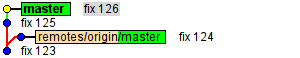
\includegraphics[width=0.7\textwidth]{./images/rebase-0.png}
  \end{center}
  \alert{git pull --rebase}
  \begin{center}
    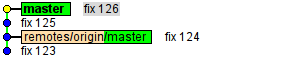
\includegraphics[width=0.7\textwidth]{./images/rebase-1.png}
  \end{center}

\end{frame}
%-------------------------------------------------------------------------------
\begin{frame}\frametitle{Rebase : danger}
Réécrire l'historique peut être lourd de conséquences !
\begin{itemize}
  \item risque de perte de commit
  \item risque d'avoir plusieurs versions d'un même commit
\end{itemize}

\end{frame}
%-------------------------------------------------------------------------------
\begin{frame}[fragile]\frametitle{Stash}
  Mettre des changements de coté: \alert{git stash}\\
\textit{to stash}: planquer, mettre dans une cachette
\end{frame}
%-------------------------------------------------------------------------------
\begin{frame}\frametitle{Dépôt central}
  \begin{center}
    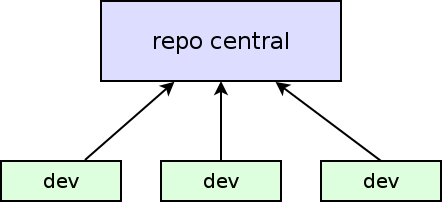
\includegraphics[width=0.7\textwidth]{./images/repo_central.png}
  \end{center}
  \begin{itemize}
    \item mise en place rapide
    \item pas de mécanisme de protection du dépôt central
  \end{itemize}

\end{frame}
%-------------------------------------------------------------------------------
\begin{frame}\frametitle{Integration manager}
  \begin{center}
    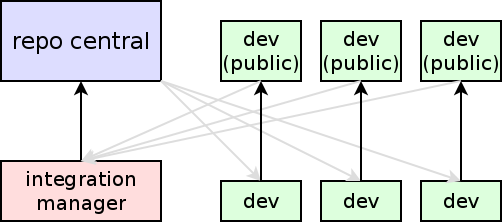
\includegraphics[width=0.7\textwidth]{./images/integration_manager.png}
  \end{center}
  \begin{itemize}
    \item plus de contrôle sur le branches du dépôt central
    \item peu adapté à des équipes importantes
  \end{itemize}

\end{frame}
%-------------------------------------------------------------------------------
\begin{frame}\frametitle{Dictateur - lieutenants}
  \begin{center}
    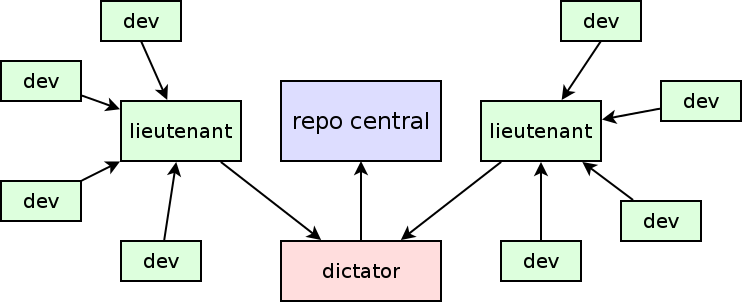
\includegraphics[width=0.8\textwidth]{./images/dictator.png}
  \end{center}
  \begin{itemize}
    \item permet de répartir les responsabilités
    \item adapté à des équipes (très) importantes
  \end{itemize}
\end{frame}

%-------------------------------------------------------------------------------
\begin{frame}\frametitle{TP : bac à sable avancé}
  rebase, reflog, stash
\end{frame}

% max 80 columns : merges become messy with pure text and longer lines.
% vim: set colorcolumn=+1 textwidth=80:

%-------------------------------------------------------------------------------
\section*{Conclusion}
% This work is licensed under the Creative Commons Attribution-NonCommercial-NoDerivs
% 3.0 Unported License. To view a copy of this license, visit
% http://creativecommons.org/licenses/by-nc-nd/3.0/ or send a letter to
% Creative Commons, 444 Castro Street, Suite 900, Mountain View, California, 94041, USA.

%-------------------------------------------------------------------------------
\begin{frame}\frametitle{En savoir plus ...}
  Docs et tutos: \url{http://gitready.com}

  Un modèle de gestion de branches: \url{http://nvie.com/posts/a-successful-git-branching-model/}

  Dépôt gratuit: \url{http://github.com/}

  Manuel Git: \url{http://schacon.github.com/git/git.html}

  En venant de SVN: \url{https://git.wiki.kernel.org/articles/g/i/t/GitSvnCrashCourse\_512d.html}

  \url{http://progit.org/}

  \url{http://www.whygitisbetterthanx.com/}

  Linus Torvalds on Git: \url{http://www.youtube.com/watch?v=4XpnKHJAok8}
\end{frame}

%-------------------------------------------------------------------------------
% max 80 columns : merges become messy with pure text and longer lines.
% vim: set colorcolumn=+1 textwidth=80:

%-------------------------------------------------------------------------------
\end{document}

% max 80 columns : merges become messy with pure text and longer lines.
% vim: set colorcolumn=+1 textwidth=80:
